% !TEX root = ../deviant.tex

\newcommand{\todofc}[1]{\todo[backgroundcolor=yellow,size=\tiny]{FC: #1}}
\newcommand{\todoinfc}[1]{\todo[inline,backgroundcolor=yellow]{FC: #1}}

\section{Experimental evaluation}
\label{sec:eval}

% Usually, an experimental evaluation of a process discovery algorithm would require to apply the proposed approach on one (or more) dataset, and to confront the learned model with those ones mined by other available approaches. However, our approach makes explicit use of information from traces labeled as ``negative'', while the totality of the approaches we could access have been designed to use positive traces only. Hence, confronting different approaches on different input data would not be fair.
% NO, questa motivazine non va bene...

One of the difficulties of evaluating process mining algorithms is that given a log, the underlying model might not be known before. As a consequence, it might be difficult to establish an \emph{ideal model} to refer and confront with. To this end, a number of metrics and evaluation indexes have been proposed in the past to evaluate how a discovered model fits a given log \todofc{Citiamo qualche metrica? O forse basta citare un paper?}. However, those metrics provide only a partial answer to the question of ``how good'' is the discovered model.\todofc{Frase molto forte, la vogliamo lasciare? FOrse dovremmo almeno citare un paper che dica qualcosa di simile\ldots}

A second issue is about the difficulty of confronting our approach with existing ones, especially if we consider that \todofc{Non so se questa cosa la voglio scrivere qui\ldots} our approach exploits information from traces labeled as ``negative'', while the majority of the approaches we could access have been designed to use positive traces only.

As a consequence, we decided to pursue two different evaluation strategies. On one side, we defined a model, and from that model we generated a synthetic, artificial log. Beside positive trace, we also generated negative traces in a controlled way, i.e. taking care that those traces violate only a small, specific and known piece of the model. Experiments conducted on that synthetic log are reported and discussed in Section \ref{sec:syntheticlog}. A first aim is to understand if our approach manages to discover a \emph{minimum} set of constraints for distinguishing positive from negative traces; a second aim is to qualitatively evaluate if the discovered model is related (and how) with the original one.

On the other side, we applied our discovery technique to some existing logs, for which results from other approaches are already available. Again, two aims: to understand weakness and strengths of our proposal w.r.t. to some relevant literature, and to confront the proposed approach with real data (and limits and difficulties that real data bring along). Section \ref{sec:realdata} is devoted to present the selected logs and discuss the obtained results.

% Such aspect is further exacerbated by the fact that our approach exploits information from traces labeled as ``negative'', while the totality of the approaches we could access have been designed to use positive traces only.



\subsection{Experiments on a synthetic dataset}
\label{sec:syntheticlog}


% \todoinfc{x Fede, Chiara DFM, Sergio: qui bisognerebbe introdurre la metodologia per provare la validit\`a del nostro approccio, cio\`e abbiamo preso questo esempio, abbiamo generato delle tracce (cit \cite{2020-Loreti}), alcune positive, altre negative che per\`o violano dei vincoli che in questo modello non sono presenti e poi abbiamo visto se riusciamo a re-impararli. Perch\`e proprio questi vincoli e non altri?}

% \subsection{Motivating example}
A bank carries out the following \emph{loan application} process\footnote{The process is inspired by the Loan Application process reported in (2018, Dumas).} in order to grant loans. The process starts when the \emph{loan application} is received. In order to decide whether to \emph{reject the application} or to \emph{send the acceptance pack} to the customer for receiving the customer's official acceptance, the bank has to \emph{assess} the \emph{eligibility} of the loan. To this aim, the customer's \emph{property} has to be \emph{appraised} and the \emph{loan risk assessed} by the bank. The bank can optionally \emph{notify} the customer about the loan \emph{approval}, of course in case the loan is not rejected. During the process the bank can also \emph{receive positive} or \emph{negative feedback} according to the experience of the loan requester. To ease the understanding of the loan application process, a Declare model of the process is reported in Fig. \ref{fig:ex}.

\begin{figure}[t]
\centering
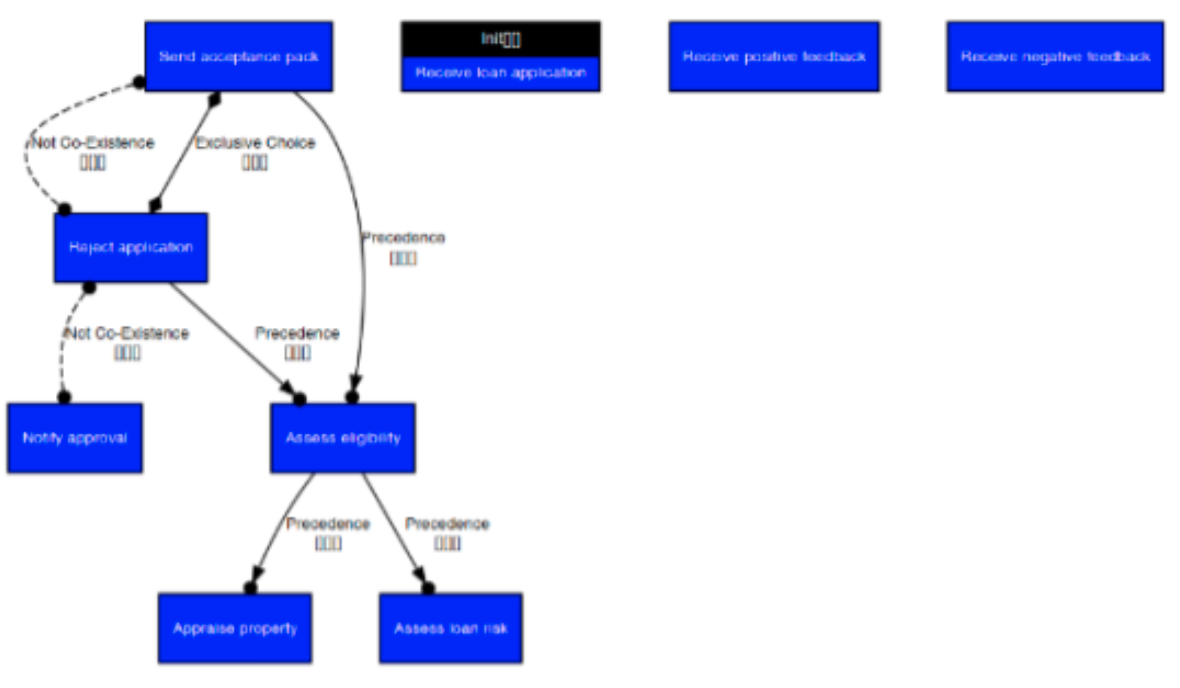
\includegraphics[width=\columnwidth]{example}
\caption{Loan approval declare process model }
\label{fig:ex}
\end{figure}

Among the processed loan application requests, some are considered as negative by the bank, while others as positive. In detail, the negative cases are the ones in which:
\begin{itemize}
\item the bank receives a negative feedback, although the acceptance pack is sent to the customer;
\item the time required for carrying out the whole procedure is huge (this happens when the property appraisal is performed after the loan risk assessment).
\end{itemize}

Being aware of the process executions that deviate from its expectations (the negative cases), the bank would like to discover a process model of the loan application procedure in which only the positive cases are included, while the deviant ones are excluded.


\subsection{Evaluation on case studies from real data}
\label{sec:realdata}

\todoindl{x Chiara DFM: questa sezione credo sia da ripopolare da capo perch\`e l'esempio \`e cambiato}

% \subsection{Results}

